\chapter{Literature Review}
\label{ch:LiteratureReview}
Stand der Forschung oder Stand der Praxis/Technik

Bezogen auf die eigenen Zielsetzungen und Fragestellungen soll aufgezeigt werden, wie andere dieses oder ähnliche Probleme gelöst haben. Worauf können Sie aufbauen, was müssen Sie neu angehen? Wodurch unterscheidet sich Ihre Lösung von anderen Lösungen? Für wissenschaftlich orientierte Arbeiten sei hier explizit auf (Balzert, S. 66 ff) verwiesen.

\section{Image Quality Assessment (IQA)}
\label{sec:OverviewTeledermatology}
In this section, the fundamentals of Image Quality Assessment (IQA) will be explored. It will introduce IQA as a field concerned with quantifying the quality of images objectively. The subsection will cover the metrics commonly used in IQA to evaluate image fidelity, clarity, and other quality aspects. Additionally, benchmark datasets utilized in IQA research and the state-of-the-art (SOTA) IQA methods will be discussed. \par
\vspace{\baselineskip}
Image Quality Assessment (IQA) is a vital process aimed at measuring various forms of degradation in images. These degradations include blur, geometric distortions such as shrinking or zooming, and blockiness artifacts resulting from compression standards. IQA primarily focuses on quantifying these degradations to ensure the fidelity and perceptual quality of images. \par
\vspace{\baselineskip}
It's worth noting that while IQA primarily measures degradation, it's closely related to other aspects of image assessment. For instance, Image Aesthetics Assessment evaluates the visual appeal of images as perceived by human eyes, which intersects with IQA. Additionally, Image Fidelity Assessment examines the accuracy of reconstructed images concerning the original view, though the primary focus of IQA remains on measuring degradation. \par

\subsection{Subjective Quality Assessment}
\label{sub:SubjectiveQualityAssessment}
Subjective quality assessment involves human observers evaluating the quality of images based on their visual perception. There are two primary methods employed: Absolute Categorical Rating and Paired Comparison. \par
\begin{itemize}
    \item Absolute Categorical Rating: In this method, human observers view an image and assign a score to its quality based on predefined categories. They evaluate the image independently without any reference image.
    \item Paired Comparison: Here, human observers compare two images: the one under assessment and a reference image. They then assign a quality score based on the perceived difference between the two images. However, Paired Comparison is not feasible in teledermatology due to the absence of a reference image, as the diagnosis of the image is unknown.
\end{itemize}
Subjective quality assessment is known for its accuracy, as it directly involves human perception. However, it is also resource and labor-intensive, requiring human assessors to evaluate each image. Moreover, subjective assessment can be prone to biases introduced by human scorers. \par

\subsection{Objective Quality Assessment}
\label{sub:ObjectiveQualityAssessment}
Objective quality assessment relies on mathematical algorithms rather than human judgment to evaluate image quality. There are three main categories of objective assessment methods: Full-Reference IQA (FR-IQA), Reduced-Reference IQA (RR-IQA), and No-Reference IQA (NR-IQA). \par
\vspace{\baselineskip}
\begin{figure}[ht]
    \centering
    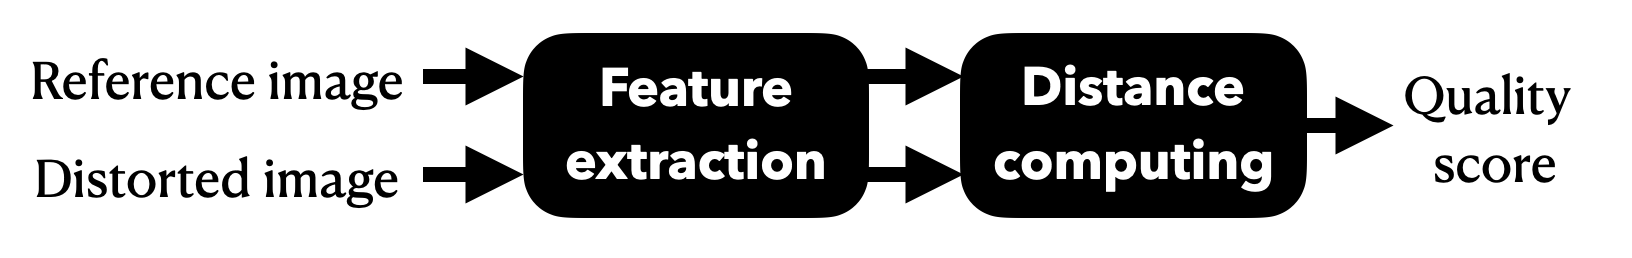
\includegraphics[keepaspectratio,width=15cm]{img/FRIQA.png}
    \caption{Comparison between a distorted image and a reference image to compute quality scores.}
    \label{fig:FRIQA}
\end{figure}
\noindent
\textbf{Full-Reference IQA (FR-IQA):} In FR-IQA \ref{fig:FRIQA}, each distorted image is compared against a reference image. Features are extracted from both images, and their distance is computed to derive a quality score. This method provides a comprehensive assessment but requires a reference image for every distorted image. \par
\vspace{\baselineskip}
\begin{figure}[ht]
    \centering
    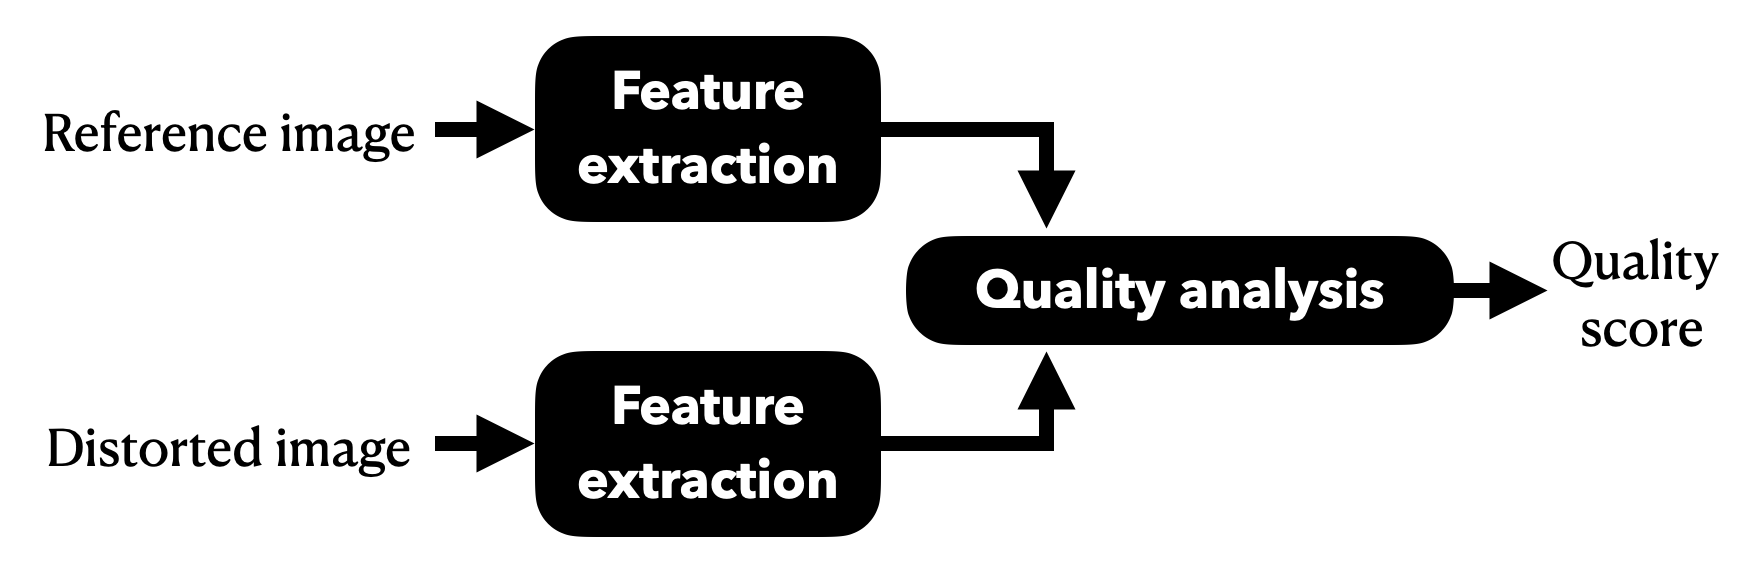
\includegraphics[keepaspectratio,width=15cm]{img/RRIQA.png}
    \caption{Reduced-reference assessment comparing features extracted from distorted and reference images for quality analysis.}
    \label{fig:RRIQA}
\end{figure}
\noindent
\textbf{Reduced-Reference IQA (RR-IQA):} RR-IQA \ref{fig:RRIQA} is similar to FR-IQA but uses a reduced sample of reference images. Features are extracted separately from the distorted image and reference images, and quality is analyzed based on these features. This approach reduces computational complexity but still requires reference information. \par
\vspace{\baselineskip}
Both FR-IQA and RR-IQA utilize two methods to analyze quality:
\begin{itemize}
    \item Spatial-Based Analysis: This method compares images pixel by pixel or region by region, offering straightforward interpretation and efficient computation. However, it may not be robust and is not directly similar to the Human Visual System (HVS).
    \item Transform-Based Analysis: Images are transformed into another domain, such as the frequency domain, mimicking the HVS. While robust, this method is complex, computationally expensive, and less intuitive to interpret.
\end{itemize}
\vspace{\baselineskip}
\begin{figure}[ht]
    \centering
    
\includegraphics[keepaspectratio,width=15cm]{img/NRIQA.png}
    \caption{Quality assessment based solely on features extracted from the distorted image, without a reference image.}
    \label{fig:NRIQA}
\end{figure}
\noindent
\textbf{No-Reference IQA (NR-IQA):} NR-IQA \ref{fig:NRIQA} does not require a reference image; only the distorted image is analyzed. Features are extracted from the distorted image, and quality is predicted based on these features. NR-IQA can focus on single distortions or be designed for general-purpose assessment, making it adaptable for diverse applications. However, it tends to be complex and computationally expensive. \par
\vspace{\baselineskip}
For this study, the focus will be on NR-IQA, particularly in the context of general-purpose quality assessment, aiming to address various distortions encountered in teledermatology images.

\subsection{Common Distortions in IQA}
\label{sub:CommonDistortionsIQA}
Image Quality Assessment (IQA) considers various distortions that affect image quality. \par
The common distortions are \cite{https://arxiv.org/abs/2310.14918}:
\begin{figure}[ht]
    \centering
    \begin{subfigure}[b]{0.24\textwidth}
        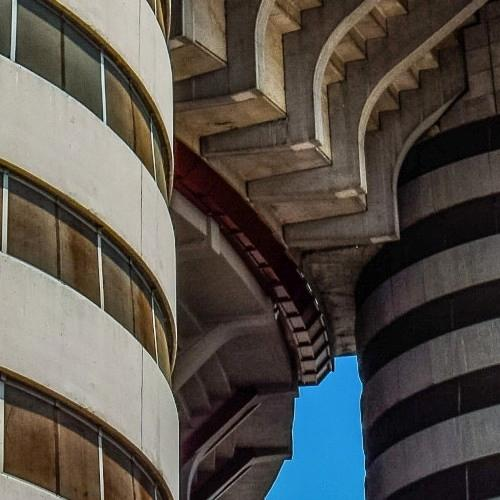
\includegraphics[width=\textwidth]{img/Original.jpg}
        \caption{Original}
    \end{subfigure}
    \hfill
    \begin{subfigure}[b]{0.24\textwidth}
        
\includegraphics[width=\textwidth]{img/Blur.jpg}
        \caption{Blur}
        \label{fig:blur}
    \end{subfigure}
    \hfill
    \begin{subfigure}[b]{0.24\textwidth}
        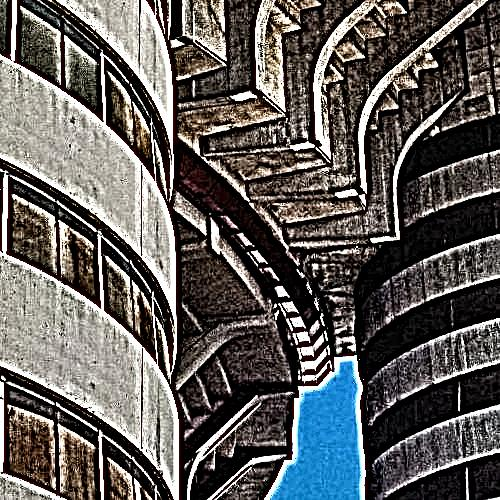
\includegraphics[width=\textwidth]{img/Sharpness.jpg}
        \caption{Sharpness}
        \label{fig:sharpness}
    \end{subfigure}
    \hfill
    \begin{subfigure}[b]{0.24\textwidth}
        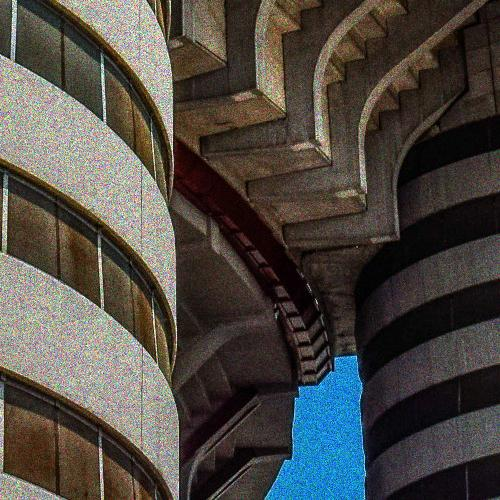
\includegraphics[width=\textwidth]{img/Noise.jpg}
        \caption{Noise}
        \label{fig:noise}
    \end{subfigure} 

    \begin{subfigure}[b]{0.24\textwidth}
        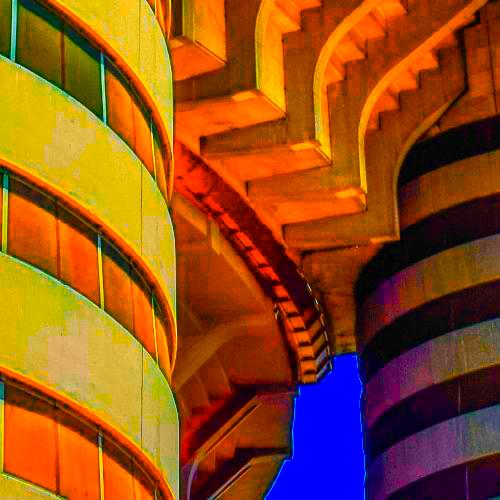
\includegraphics[width=\textwidth]{img/ColorAccuracy.jpg}
        \caption{Color Accuracy}
        \label{fig:color_accuracy}
    \end{subfigure}
    \hfill
    \begin{subfigure}[b]{0.24\textwidth}
        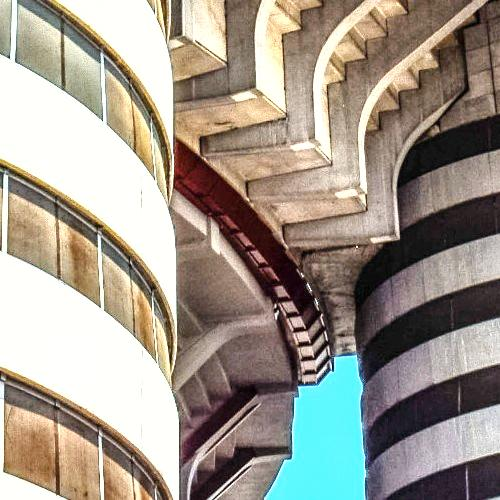
\includegraphics[width=\textwidth]{img/BrightnessContrast.jpg}
        \caption{Brightness \& Contrast}
        \label{fig:brightness_contrast}
    \end{subfigure}
    \hfill
    \begin{subfigure}[b]{0.24\textwidth}
        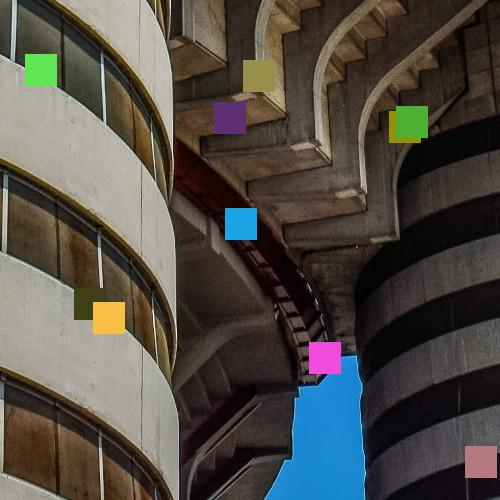
\includegraphics[width=\textwidth]{img/Artifacts.jpg}
        \caption{Artifacts}
        \label{fig:artifacts}
    \end{subfigure}
    \hfill
    \begin{subfigure}[b]{0.24\textwidth}
        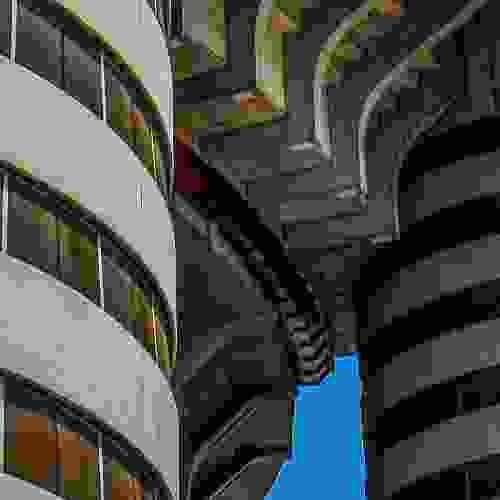
\includegraphics[width=\textwidth]{img/Compression.jpg}
        \caption{Compression}
        \label{fig:compression}
    \end{subfigure}
    \caption{Example images illustrating common distortions used in Image Quality Assessment.}
    \label{fig:distortions}
\end{figure}
\begin{enumerate}
    \item \textbf{Blur}: Blurred images lack sharpness and clarity, often resulting from motion blur, focus issues, or lens imperfections. Example Image: \ref{fig:blur}.
    
    \item \textbf{Sharpness}: Sharpness refers to the clarity and definition of edges and details in an image. Example Image: \ref{fig:sharpness}.
    
    \item \textbf{Noise}: Noise manifests as random variations in brightness or color in an image, typically caused by sensor limitations or high ISO settings. Example Image: \ref{fig:noise}.
    
    \item \textbf{Color Accuracy}: Color accuracy pertains to the faithful reproduction of colors in an image. Distortions in color accuracy can lead to inaccurate or unrealistic color representation. Example Image: \ref{fig:color_accuracy}.
    
    \item \textbf{Brightness \& Contrast}: Brightness refers to the overall lightness or darkness of an image, while contrast relates to the difference in luminance between the lightest and darkest parts. Distortions in brightness and contrast can result in images appearing too dark, too bright, or lacking in tonal range. Example Image: \ref{fig:brightness_contrast}.
    
    \item \textbf{Artifacts}: Artifacts are unwanted visual anomalies introduced during image acquisition or processing, such as compression artifacts, halos, or jagged edges. Example Image: \ref{fig:artifacts}.
    
    \item \textbf{Compression}: Compression distortions occur when an image is compressed to reduce file size, leading to loss of detail and image degradation. Example Image: \ref{fig:compression}.
\end{enumerate}
Each distortion type affects the visual quality and perceptual fidelity of images, influencing the effectiveness of IQA methodologies in assessing image quality. Understanding these distortions is crucial for developing robust quality assessment algorithms and enhancing image fidelity in various applications, including teledermatology.

\subsection{Benchmark Datasets for IQA}
\label{sub:BenchmarkDatasetsIQA}
Benchmark datasets play a crucial role in advancing the field of Image Quality Assessment (IQA) by providing standardized and diverse sets of images with known distortions and corresponding quality annotations. These datasets serve as reference points for evaluating the performance of IQA algorithms and comparing their effectiveness across different distortion types, levels, and image characteristics. \par

By offering a wide range of images spanning various content types, resolutions, and distortion scenarios, benchmark datasets enable researchers to rigorously assess the robustness, accuracy, and generalization capability of IQA methodologies. Furthermore, these datasets facilitate the development of novel algorithms by providing ground-truth quality scores and fostering reproducible research practices. \par

In the following sections, we will explore some prominent benchmark datasets commonly used in the field of IQA, highlighting their key characteristics, contents, and contributions to advancing the state-of-the-art in image quality assessment. \par

\begin{table*}[!t]
    \centering
    \caption{An overview of IQA databases}
    \label{tab:iqa_databases}
    \setlength{\tabcolsep}{0.3em}
    \scalebox{0.57}{
    \renewcommand{\arraystretch}{1.5}
    \begin{tabular}{p{1.8cm} p{2cm} c c c c c c c}
    \toprule
        Category & Database & Year & \#Ref. & \#Dist. & \#Dist. Type & \#Dist. Level & Resolution Type & Ground-truth \\
        \hline
        \multirow{10}{*}{General} 
        & LIVE \cite{LIVE} & 2004 & 30 & 779 & 5 & 5 or 4 & 768 x 512 & DMOS \\
        & TID2008 \cite{TID2008} & 2008 & 25 & 1700 & 17 & 4 & 512 x 384 & MOS \\
        & TID2013 \cite{TID2013} & 2013 & 25 & 3000 & 24 & 5 & 512 x 384 & MOS \\
        & CSIQ \cite{CSIQ} & 2009 & 30 & 866 & 6 & 5 or 4 & 512 x 512 & DMOS \\
        & IVC \cite{IVC} & 2005 & 10 & 54 & 4 & 5 & 512 x 512 & MOS \\
        & MICT \cite{MICT} & 2001 & 14 & 168 & 2 & 6 & 768 x 512 & MOS \\
        & A57 \cite{A57} & 2007 & 3 & 54 & 6 & 3 & 512 x 512 & MOS \\
        & WED \cite{WED} & 2017 & 4744 & 94880 & 4 & 5 & - & - \\
        & KADIS700K \cite{KADIS700K} & - & - & - & - & - & - & - \\
        & KADID \cite{KADID} & - & - & - & - & - & - & - \\
        \hline
        \multirow{3}{*}{Multiple Distortions} 
        & LIVEMD \cite{LIVEMD} & 2012 & 15 & 405 & 2 & - & 1280 x 720 & DMOS \\
        & MDID2013 \cite{MDID2013} & 2013 & 12 & 324 & - & - & 768 x 512 or 1280 x 720 & DMOS \\
        & MDID2016 \cite{MDID2016} & 2016 & 20 & 1600 & - & - & 512 x 384 & MOS \\
        \hline
        \multirow{4}{*}{Screen content} 
        & SIQAD \cite{SIQAD} & 2014 & 20 & 980 & 7 & 7 & 700 x 700 & DMOS \\
        & SCIQ \cite{SCIQ} & 2017 & 40 & 1800 & 9 & 5 & 1280 x 720 & MOS \\
        & CCT \cite{CCT} & 2017 & 72 & 1320 & 2 & 11 & 1280 x 720 to 1920 x 1080 & MOS \\
        & HSNID \cite{HSNID} & 2019 & 20 & 600 & 6 & 5 &  - & MOS \\
        \hline
        \multirow{2}{*}{Authentic} 
        & LIVE Wild \cite{LIVEWild} & 2016 & 0 & 1162 & - & - & 500 x 500 & MOS \\
        & CID2013 \cite{CID2013} & 2015 & 0 & 480 & - & - & 1600 x 1200 & MOS \\
    \bottomrule
    \end{tabular}
    }
\end{table*}
\vspace{\baselineskip}
\textbf{Traditional IQA Databases}
\todo{Fill out Dist. Type in Table}
\begin{itemize}
    \item \textbf{LIVE image quality assessment database} \cite{LIVE}: LIVE includes 29 pristine images and 779 distorted images corrupted by 5 types of distortions: JPEG compression (JPEG), JPEG2000 compression (JP2K), white noise (WN), Gaussian blur (GB), and simulated fast fading Rayleigh channel (FF). Each distortion type contains 5 or 4 distortion levels. Most images are 768 $\times$ 512 pixels in size.
    \item \textbf{Tampere image database 2008 (TID2008)} \cite{TID2008}: TID2008 includes 25 pristine images and 1700 distorted images corrupted by 17 types of distortions, with 4 levels for each distortion type. All images have a fixed resolution of 512 $\times$ 384.
    \item \textbf{Tampere image database 2013 (TID2013)} \cite{TID2013}: TID2013 is extended from TID2008 by increasing the number of distortion levels to 5, and the number of distortion types to 24. Therefore, 3000 distorted images are generated from 25 pristine images. The subjective testing and data processing steps are similar to that of TID2008.
    \item \textbf{Categorical subjective image quality (CSIQ) database} \cite{CSIQ}: It contains 30 pristine images and 866 distorted images corrupted by JPEG, JP2K, WN, GB, additive pink Gaussian noise, and global contrast decrements, with 5 or 4 levels for each distortion type. The resolution is 512 $\times$ 512.
    \item \textbf{IRCCyN/IVC subjective quality assessment database} \cite{IVC}: IVC consists of 10 pristine images and 235 distorted images corrupted by JPEG, JP2K, blur, and locally adaptive resolution coding, with 5 levels for each distortion type. The resolution is fixed at 512 $\times$ 512.
    \item \textbf{MICT image quality evaluation database} \cite{MICT}: MICT includes 14 pristine images and 168 distorted images corrupted by JPEG and JP2K, with 6 levels for each distortion type. The resolution is 768 $\times$ 512.
    \item \textbf{A57 database} \cite{A57}: A57 includes 3 pristine images and 54 distorted images corrupted by 6 types of distortions, with 3 levels for each distortion type. All images are in gray scale. The resolution is 512 $\times$ 512.
    \item \textbf{Waterloo exploration database (WED)} \cite{WED}: WED includes 4744 pristine natural images and 94880 distorted images corrupted by JPEG, JP2K, GB, and WN, with 5 levels for each distortion type. The images have various resolutions. No human opinion score is provided, but the authors introduce several alternative test criteria to evaluate the IQA models.
\end{itemize}

\textbf{Multiple Distortions IQA Databases}
\begin{itemize}
    \item \textbf{LIVE multiply distorted (LIVEMD) database} \cite{LIVEMD}: LIVEMD consists of 15 reference images and 405 multiply distorted images. The database includes one/double-fold artifacts. Each multiply distorted image is corrupted under two multiple distortion scenarios: Gaussian blur followed by JPEG and Gaussian blur followed by white noise. All images have a resolution of 1280 $\times$ 720.
    \item \textbf{Multiply distorted image database 2013 (MDID2013)} \cite{MDID2013}: MDID2013 has a total of 12 pristine images and 324 distorted images. Each pristine image is corrupted successively by Gaussian blur, white noise, and JPEG. The images have resolutions of 768 $\times$ 512 or 1280 $\times$ 720.
    \item \textbf{Multiply distorted image database 2016 (MDID2016)} \cite{MDID2016}: MDID2016 consists of 20 reference images and 1600 distorted images. Five distortion types are introduced, i.e., white noise, Gaussian blur, JPEG, JPEG2000, and contrast change (CC). The order of distortions is as follows: Gaussian blur or CC first, JPEG or JPEG2000 second, and white noise last. All distorted images are with random types and levels of distortions. The image resolution is 512 $\times$ 384.
\end{itemize}

\textbf{Screen Content IQA Databases}
\begin{itemize}
    \item \textbf{Screen Image Quality Assessment Database (SIQAD)} \cite{SIQAD}: SIQAD includes 20 pristine and 980 distorted screen content images (SCIs). Distortion types include white noise (WN), Gaussian blur (GB), color cast (CC), JPEG, JPEG2000 (JP2K), motion blur (MB), and layer segmentation-based compression, with 7 levels for each type. The images have various resolutions near 700 $\times$ 700.
    \item \textbf{Screen Content Image Quality (SCIQ) Database} \cite{SCIQ}: SCIQ consists of 40 pristine and 1800 distorted SCIs corrupted by 9 types of distortions, including WN, GB, MB, CC, JPEG, JP2K, color saturation change (CSC), color quantization with dithering (CQD), and the screen content coding extension of High Efficiency Video Coding (HEVC-SCC). Five distortion levels are considered. The resolution is fixed at 1280 $\times$ 720.
    \item \textbf{Cross-Content-Type (CCT) Database} \cite{CCT}: CCT is constructed to conduct cross-content-type IQA research. CCT consists of 72 pristine and 1320 distorted natural scene images (NSIs), computer graphic images (CGIs), and SCIs. Two distortion types are considered, i.e., HEVC and HEVC-SCC coding, with 11 distortion levels for each type. The image resolution is either 1920 $\times$ 1080 or 1280 $\times$ 720.
    \item \textbf{Hybrid Screen Content and Natural Scene Image Database (HSNID)} \cite{HSNID}: HSNID has 10 pristine NSIs and 10 pristine SCIs, and 600 distorted NSIs and SCIs corrupted by WN, GB, MB, CC, JPEG, and JP2K, with 5 distortion levels for each type.
\end{itemize}

\textbf{Authentic Distortions IQA Databases}
\begin{itemize}
    \item \textbf{LIVE in the wild image quality challenge database} \cite{LIVEWild}: It includes 1162 authentically distorted images captured using a variety of mobile devices. Complex real distortions, which are not well-modeled by the synthetic distortions are included. All images are cropped to the resolution of 500 $\times$ 500. MOSs collected via crowdsourcing are provided.
    \item \textbf{Camera image database (CID2013)} \cite{CID2013}: CID2013 is designed to test no-reference IQA algorithms. It includes 480 real images captured from 8 typical scenes using 79 consumer cameras and mobile phones. The images are rated from 5 aspects: the overall quality, sharpness, graininess, lightness, and color saturation scales. The images are scaled to a size of 1600 $\times$ 1200.
\end{itemize}


\subsection{State-of-the-Art in IQA}
\label{sub:SOTA_IQA}
The current state-of-the-art (SOTA) in Image Quality Assessment (IQA) within the general image domain is ARNIQA. ARNIQA stands out for its ability to learn the distortion manifold encompassing all possible image degradations. It has demonstrated superiority in handling both synthetic and authentic distortions. \par
\vspace{\baselineskip}
ARNIQA comprises three main components:

\textbf{Image Degradation Model:} This component synthetically degrades images using an extensive set of 1.9 billion distinct degradation combinations. It can randomly stack up to 7 degradations across different ranges, enabling comprehensive coverage of possible distortions. \par
\textbf{SimCLR (Simple Framework for Contrastive Learning):} SimCLR extracts features from an unsupervised setting, learning meaningful representations of data and capturing essential patterns and relationships within the dataset. Notably, it can be reused without retraining as a backbone for various tasks. \par
\textbf{Linear Regressor:} A simple linear regressor maps the learned representations to quality scores ranging from 0 to 1. Similar degrees and patterns of degradation result in similar quality scores, indicating their relative positions in the distortion manifold. \par
\vspace{\baselineskip}
ARNIQA offers several advantages over previous methods. It is less complex, making it more accessible and easier to implement. Additionally, it is data-efficient, exhibiting strong generalization capabilities across diverse datasets and applications. Furthermore, ARNIQA is robust, reliably delivering accurate quality assessments across a wide range of distortion types and severities. \par
\vspace{\baselineskip}
SimCLR Explanation: SimCLR employs a unique approach to learn meaningful representations of data by maximizing the similarity between different views of the same image while maximizing the dissimilarity between views of different images. By focusing on inherent distortions rather than image content, SimCLR disregards irrelevant details, enhancing its robustness. Moreover, SimCLR employs a strategy to augment the dataset by generating hard negative examples, which helps improve model performance and generalization. \par

\subsection{Challenges and Opportunities in IQA}
\label{sub:ChallengesOpportunitiesIQA}
Despite advancements, IQA faces challenges such as subjective perception, computational complexity, and the need for robust evaluation methodologies. However, ongoing research presents opportunities for addressing these challenges and further improving the effectiveness and efficiency of IQA methods. \par
\vspace{\baselineskip}
\noindent


\section{Teledermatology}
\label{sec:Teledermatology}
The following section provides an overview of teledermatology, a specialized field of dermatology that utilizes telecommunications technology to provide remote diagnosis and consultation for skin conditions. This section discusses the importance of image quality in teledermatology, quality criteria for teledermatology images, as well as challenges and opportunities associated with the practice. \par
\vspace{\baselineskip}
\noindent

\subsection{Introduction to Teledermatology}
\label{sub:IntroductionTeledermatology}
The term "teledermatology" combines "tele", which refers to distance or remote communication, and "dermatology", the medical field focused on skin health. This specialized branch of dermatolgoy utilizes telecommunications technology to provide remote diagnosis and consultation for skin conditions.\par
\vspace{\baselineskip}
\noindent
This innovative approach to healthcare delivery is particularly beneficial for patients in remote or underserved areas, as well as for those with mobility issues. Teledermatology services can be provided in real-time, or through store and forward images, wherein the patient captures images of their skin or any skin-related issues using a camera or smartphone and send them electronically to a dermatologist, along with relevant details about their condition, such as symptoms and medical history. This allows dermatologists to assess the skin condition remotely and provide recommendations or treatment plans without the need for an in-person visit.\par

\subsection{Importance of Image Quality in Teledermatology}
\label{sub:ImportanceIQA_Teledermatology}
High-quality images are essential for accurate diagnosis in teledermatology. While poor image quality can lead to misinterpretation of skin lesions, incorrect diagnosis or missed diagnosis. \par
\vspace{\baselineskip}
\noindent
With good image quality the dermatologists can better assess the severity of skin conditions and formulate appropriate treatment plans.\par
\vspace{\baselineskip}
\noindent
No in-persons visits and improve accessibility to specialized care.\par
\vspace{\baselineskip}
\noindent
Maintaining consistent image quality standards ensures the reliablility and reproducibility of teledermatology services. It minimizes variability and enhances the overall reliability of remote diagnosis and consultation process\par
\vspace{\baselineskip}
\noindent
show good and bad quality images!!\par

\subsection{Quality Criteria for Teledermatology Images}
\label{sub:QualityCriteriaTeledermatology}
In the context of teledermatology, Image Quality Assessment (IQA) must consider specific criteria to ensure accurate diagnosis and effective remote consultations. These quality criteria include:

\begin{enumerate}
    \item \textbf{Lighting}: Position the light source evenly to avoid shadows and overexposure. Natural light or diffused artificial light can help illuminate the skin lesion uniformly and reduce glare.
    \item \textbf{Background}: Use a plain, non-reflective background to minimize distractions and ensure the focus remains on the skin lesion. A neutral-colored backdrop, such as white or gray, is ideal for providing contrast with the lesion.
    \item \textbf{Field of View}: Center the skin lesion or area of interest within the frame to ensure complete coverage and avoid cutting off important details. Maintain a consistent distance between the camera and the skin to prevent distortion.
    \item \textbf{Orientation}: Orient the camera perpendicular to the skin surface to capture images in the correct orientation. Align the camera with the skin lesion to maintain consistency and facilitate accurate comparison between images.
    \item \textbf{Focus \& Depth of Field}: Ensure the camera is in focus and adjust the aperture to achieve sufficient depth of field. Focus on the skin lesion to capture sharp, detailed images without blurriness or loss of clarity.
    \item \textbf{Resolution}: Use a camera with high-resolution capabilities to capture fine details and nuances of the skin lesion. Adjust the camera settings to the highest resolution possible to ensure clarity and precision in the image.
    \item \textbf{Color Calibration}: Calibrate the camera settings to accurately reproduce colors and skin tones. Avoid harsh lighting or color casts that may distort the color representation of the skin lesion. Use a color reference chart or white balance settings to ensure color accuracy.
\end{enumerate}
By following these guidelines, clinicians and patients can capture high-quality images that meet the necessary standards for accurate diagnosis and effective remote consultations in teledermatology.


\subsection{Challenges and Opportunities in Teledermatology}
\label{sub:ChallengesOpportunitiesTeledermatology}
Challenges: picture taken by the patient is not in a good qualtiy, patient data security and privacy, including compliance with regulations. The whole patient cannot be examined, only localised. No touching of skin. Demands diligence in documentation, storage and consent. Who has the clinical accountability or responsibility. Double charging. Teledermatology is not included in training curriculum for doctors. Different patient experience. Barriers in practice such as individual preference of doctors, resistance to change and no benefit in investing time to adapt. \par
\vspace{\baselineskip}
\noindent
Opportunities: increase access to care, reduce waiting times, reduce travel time and costs, increase patient satisfaction, increase efficiency, increase access to specialist care, increase access to education and training, increase access to research and clinical trials, increase access to data and analytics, increase access to technology and innovation, increase access to collaboration and networking, increase access to telemedicine and telehealth. \par

\subsection{Previous Research in Teledermatology}
\label{sub:PreviousResearchTeledermatology}
The article by Primary Care Commissioning in 2011 outlined quality standards for teledermatology services using store and forward images. These standards include: \par
\noindent
\begin{itemize}
    \item Standard 1: Models of teledermatology services including links to other services
    \item Standard 2: Selecting patients for teledermatology
    \item Standard 3: Gaining the patient's informed consent
    \item Standard 4: Competent staff
    \item Standard 5: The teledermatology referral: patient history and suitable images
    \item Standard 6: Communication between referring and reporting clinician
    \item Standard 7: Information governance and record-keeping
    \item Standard 8: Audit and quality control
\end{itemize}
\par
\noindent
These standards serve as guidelines for ensuring the quality and effectiveness of teledermatology services, particularly in the context of using store and forward images.